%----------------------------------------------------------------------------------------
% preamble.tex: パッケージの読み込みと基本設定
%----------------------------------------------------------------------------------------

% --- hyperref の事前設定(衝突回避のためパッケージ読み込み前に実行) ---
\PassOptionsToPackage{unicode=true,colorlinks=true,linkcolor=blue,urlcolor=blue}{hyperref} 

% --- 日本語設定 (LuaTeX-ja) ---
\usepackage{luatexja} 
\usepackage{luatexja-fontspec} 
\usepackage{luatexja-ruby} 
\setsansjfont{Hiragino Sans}[BoldFont={Hiragino Sans W6}] 

% --- 基本パッケージ ---
\usepackage[table]{xcolor} 
\usepackage{graphicx} 
\usepackage[absolute,overlay]{textpos} 
\usepackage[abs]{overpic} 
\usepackage{tikz} 
\usetikzlibrary{positioning, shapes.geometric, calc, backgrounds} 
\usepackage{array} 
\usepackage{tabularx} 
\usepackage{booktabs} 
\usepackage{makecell} 
\usepackage{mathtools} 
\usepackage{longtable} 
\usepackage{pdfpages} 
\usepackage{etoolbox} 
\usepackage[normalem]{ulem} 
\usepackage{pgf} 

% --- コード表示 (minted) ---
\usepackage{minted} 
\setminted{ 
  frame=single, 
  framesep=2mm, 
  fontsize=\footnotesize, 
  breaklines=true 
} 

% --- 装飾ボックス (tcolorbox) ---
\usepackage[most]{tcolorbox} 
\tcbuselibrary{skins, raster} 

% --- 外部パッケージ・設定ファイルの読み込み ---
\usepackage{teacherframe} 
% grid_debug.tex  ---  グリッド表示マクロ

\newcommand{\showgrid}{%
\begin{tikzpicture}[remember picture,overlay]
  \draw[step=1cm,gray!25] (current page.south west) grid (current page.north east);
  \fill[red] (current page.north west) circle (2pt);
  \fill[red] (current page.north east) circle (2pt);
  \fill[red] (current page.south west) circle (2pt);
  \fill[red] (current page.south east) circle (2pt);
\end{tikzpicture}%
} 

% --- 最後に読み込むべきパッケージ ---
\usepackage{hyperref}